\documentclass{report}
\usepackage{graphicx, tikz-cd, float, titlepic, booktabs} % Required for inserting images
\usepackage{pgfplots}
\pgfplotsset{compat=1.15}
\usepackage{mathrsfs}
\usetikzlibrary{arrows}
\usepackage{amsmath, amssymb, amsthm, amsfonts, siunitx, physics, gensymb}
\AtBeginDocument{\RenewCommandCopy\qty\SI}
\usepackage[version=4]{mhchem}
\usepackage[most,many,breakable]{tcolorbox}
\usepackage{xcolor, fancyhdr, varwidth}
\usepackage[Glenn]{fncychap}
%Options: Sonny, Lenny, Glenn, Conny, Rejne, Bjarne, Bjornstrup
\usepackage{hyperref, cleveref}
\usepackage{icomma, enumitem} %comma as decimal and continue enumerate with [resume]
\usepackage{plimsoll} %use standard state symbol with \stst
\usepackage[danish]{babel}
%%%%%%%%%%%%%%%%%%%%%%%%%%%%%%
% SELF MADE COLORS
%%%%%%%%%%%%%%%%%%%%%%%%%%%%%%
\definecolor{myg}{RGB}{56, 140, 70}
\definecolor{myb}{RGB}{45, 111, 177}
\definecolor{myr}{RGB}{199, 68, 64}
\definecolor{mytheorembg}{HTML}{F2F2F9}
\definecolor{mytheoremfr}{HTML}{00007B}
\definecolor{mylenmabg}{HTML}{FFFAF8}
\definecolor{mylenmafr}{HTML}{983b0f}
\definecolor{mypropbg}{HTML}{f2fbfc}
\definecolor{mypropfr}{HTML}{191971}
\definecolor{myexamplebg}{HTML}{F2FBF8}
\definecolor{myexamplefr}{HTML}{88D6D1}
\definecolor{myexampleti}{HTML}{2A7F7F}
\definecolor{mydefinitbg}{HTML}{E5E5FF}
\definecolor{mydefinitfr}{HTML}{3F3FA3}
\definecolor{notesgreen}{RGB}{0,162,0}
\definecolor{myp}{RGB}{197, 92, 212}
\definecolor{mygr}{HTML}{2C3338}
\definecolor{myred}{RGB}{127,0,0}
\definecolor{myyellow}{RGB}{169,121,69}
\definecolor{myexercisebg}{HTML}{F2FBF8}
\definecolor{myexercisefg}{HTML}{88D6D1}
%%%%%%%%%%%%%%%%%%%%%%%%%%%%%%%%%%%%%%%%%%%%%%%%%%%%%%%%%%%%%%%%%%%%%%
% Box environments for theorems and problems
%%%%%%%%%%%%%%%%%%%%%%%%%%%%%%%%%%%%%%%%%%%%%%%%%%%%%%%%%%%%%%%%%%%%%
\setlength{\parindent}{1cm}
%================================
% Question BOX
%================================
\makeatletter
\newtcbtheorem{question}{Opgave}{enhanced,
	breakable,
	colback=white,
	colframe=myb!80!black,
	attach boxed title to top left={yshift*=-\tcboxedtitleheight},
	fonttitle=\bfseries,
	title={#2},
	boxed title size=title,
	boxed title style={%
			sharp corners,
			rounded corners=northwest,
			colback=tcbcolframe,
			boxrule=0pt,
		},
	underlay boxed title={%
			\path[fill=tcbcolframe] (title.south west)--(title.south east)
			to[out=0, in=180] ([xshift=5mm]title.east)--
			(title.center-|frame.east)
			[rounded corners=\kvtcb@arc] |-
			(frame.north) -| cycle;
		},
	#1
}{def}
\makeatother
%================================
% DEFINITION BOX
%================================

\newtcbtheorem[]{Definition}{Definition}{enhanced,
	before skip=2mm,after skip=2mm, colback=red!5,colframe=red!80!black,boxrule=0.5mm,
	attach boxed title to top left={xshift=1cm,yshift*=1mm-\tcboxedtitleheight}, varwidth boxed title*=-3cm,
	boxed title style={frame code={
					\path[fill=tcbcolback]
					([yshift=-1mm,xshift=-1mm]frame.north west)
					arc[start angle=0,end angle=180,radius=1mm]
					([yshift=-1mm,xshift=1mm]frame.north east)
					arc[start angle=180,end angle=0,radius=1mm];
					\path[left color=tcbcolback!60!black,right color=tcbcolback!60!black,
						middle color=tcbcolback!80!black]
					([xshift=-2mm]frame.north west) -- ([xshift=2mm]frame.north east)
					[rounded corners=1mm]-- ([xshift=1mm,yshift=-1mm]frame.north east)
					-- (frame.south east) -- (frame.south west)
					-- ([xshift=-1mm,yshift=-1mm]frame.north west)
					[sharp corners]-- cycle;
				},interior engine=empty,
		},
	fonttitle=\bfseries,
	title={#2},#1}{def}
\newtcbtheorem[]{definition}{Definition}{enhanced,
	before skip=2mm,after skip=2mm, colback=red!5,colframe=red!80!black,boxrule=0.5mm,
	attach boxed title to top left={xshift=1cm,yshift*=1mm-\tcboxedtitleheight}, varwidth boxed title*=-3cm,
	boxed title style={frame code={
					\path[fill=tcbcolback]
					([yshift=-1mm,xshift=-1mm]frame.north west)
					arc[start angle=0,end angle=180,radius=1mm]
					([yshift=-1mm,xshift=1mm]frame.north east)
					arc[start angle=180,end angle=0,radius=1mm];
					\path[left color=tcbcolback!60!black,right color=tcbcolback!60!black,
						middle color=tcbcolback!80!black]
					([xshift=-2mm]frame.north west) -- ([xshift=2mm]frame.north east)
					[rounded corners=1mm]-- ([xshift=1mm,yshift=-1mm]frame.north east)
					-- (frame.south east) -- (frame.south west)
					-- ([xshift=-1mm,yshift=-1mm]frame.north west)
					[sharp corners]-- cycle;
				},interior engine=empty,
		},
	fonttitle=\bfseries,
	title={#2},#1}{def}

\newtcbtheorem{theo}%
    {Theorem}{}{theorem}
\newtcolorbox{prob}[1]{colback=red!5!white,colframe=red!50!black,fonttitle=\bfseries,title={#1}}
%================================
% NOTE BOX
%================================

\usetikzlibrary{arrows,calc,shadows.blur}
\tcbuselibrary{skins}
\newtcolorbox{note}[1][]{%
	enhanced jigsaw,
	colback=gray!20!white,%
	colframe=gray!80!black,
	size=small,
	boxrule=1pt,
	title=\textbf{Note:},
	halign title=flush center,
	coltitle=black,
	breakable,
	drop shadow=black!50!white,
	attach boxed title to top left={xshift=1cm,yshift=-\tcboxedtitleheight/2,yshifttext=-\tcboxedtitleheight/2},
	minipage boxed title=1.5cm,
	boxed title style={%
			colback=white,
			size=fbox,
			boxrule=1pt,
			boxsep=2pt,
			underlay={%
					\coordinate (dotA) at ($(interior.west) + (-0.5pt,0)$);
					\coordinate (dotB) at ($(interior.east) + (0.5pt,0)$);
					\begin{scope}
						\clip (interior.north west) rectangle ([xshift=3ex]interior.east);
						\filldraw [white, blur shadow={shadow opacity=60, shadow yshift=-.75ex}, rounded corners=2pt] (interior.north west) rectangle (interior.south east);
					\end{scope}
					\begin{scope}[gray!80!black]
						\fill (dotA) circle (2pt);
						\fill (dotB) circle (2pt);
					\end{scope}
				},
		},
	#1,
}
%================================
% EXAMPLE BOX
%================================
\newtcbtheorem[number within=section]{Example}{Example}
{%
	colback = myexamplebg
	,breakable
	,colframe = myexamplefr
	,coltitle = myexampleti
	,boxrule = 1pt
	,sharp corners
	,detach title
	,before upper=\tcbtitle\par\smallskip
	,fonttitle = \bfseries
	,description font = \mdseries
	,separator sign none
	,description delimiters parenthesis
}
{ex}
%================================
% THEOREM BOX
%================================

\tcbuselibrary{theorems,skins,hooks}
\newtcbtheorem[number within=section]{Theorem}{Theorem}
{%
	enhanced,
	breakable,
	colback = mytheorembg,
	frame hidden,
	boxrule = 0sp,
	borderline west = {2pt}{0pt}{mytheoremfr},
	sharp corners,
	detach title,
	before upper = \tcbtitle\par\smallskip,
	coltitle = mytheoremfr,
	fonttitle = \bfseries\sffamily,
	description font = \mdseries,
	separator sign none,
	segmentation style={solid, mytheoremfr},
}
{th}

%%%%%%%%%%%%%%%%%%%%%%%%%%%%%%%%%%%%%%%%%%%%%%%%%%%%%%%%%%%%%%%%%
% SELF MADE COMMANDS
%%%%%%%%%%%%%%%%%%%%%%%%%%%%%%
\newcommand{\sol}{\setlength{\parindent}{0cm}\textbf{\textit{Løsning:}}\setlength{\parindent}{1cm}}
%%%%%%%%%%%%%%%%%%%%%%%%%%%%%%%%%
\usepackage[tmargin=2cm,rmargin=1in,lmargin=1in,margin=0.85in,bmargin=2cm,footskip=.2in]{geometry}\pagestyle{fancy}
\lhead{Minrui Kevin Zhou 3.b}
\rhead{H3: Mekanik}

\title{H3: Mekanik – cirkelbevægelse\\
{\Large \textbf{3.b mat A}}}
\author{Kevin Zhou}
\date{\today}

\begin{document}
\maketitle
\section*{Bobslæde}
\sol \\
\textbf{a.}
Hvis man ser bort fra alle friktionskræfter, er det kun tyngdekraften $\overrightarrow{\textbf{F}_t}$ og normalkraften $\overrightarrow{\textbf{F}_N}$, der påvirker bobslæden.
Den eneste ydre kraft er da $\overrightarrow{\textbf{F}_N}$.
Siden denne altid er vinkelret med bobslædens retning, så må der gælde, at
\begin{equation*}
\begin{split}
  \Delta E_{\text{mek} }&=A_{\text{ydre} }\\
  &=|\overrightarrow{\textbf{F}_N} | \cdot \Delta s \cdot \cos\left(90 \degree \right) \\
  &=0
\end{split}
\end{equation*}
Tilvæksten i mekanisk energi er altså 0. 
Per definition har vi $E _{\text{mek} }=E _{\text{kin} }+E _{\text{pot} }$, hvor $E _{\text{kin} }=0$ ved toppen og bobslæden opnår maksimal fart når $E _{\text{pot} }=0$. 
Altså har vi
\begin{equation*}
\begin{split}
  0+m \cdot g \cdot h=\frac{1}{2} \cdot m \cdot v^2 +0 \iff v=\sqrt{2 \cdot g \cdot h} 
\end{split}
\end{equation*}
da vi lader farten være en positiv størrelse.
Da vi kender højden, kan vi nu udregne farten.
\begin{equation*}
\begin{split}
  v&=\sqrt{2 \cdot g \cdot h} \\
  &=\sqrt{2 \cdot 9,82 \;\unit{m/s^2} \cdot 114,3 \;\unit{m} } \\
  &\approx 47,4 \;\unit{m/s} \\
\end{split}
\end{equation*}
Bobslædens maksimale fart på banen, hvis man ser bort fra friktionskræfter er altså $47,4 \;\unit{m/s} $.\\[1ex]
\textbf{b.}
Fra \textbf{a.} har vi allerede, at normalkraftens arbejde er 0.
Både gnidningskraften $\overrightarrow{\textbf{F}_{\mu}} $ og luftmodstanden $\overrightarrow{\textbf{F}_{\text{luft}}}$ er ydre kræfter, der er modsatrettet bobslædens retning, og vi har igen
\begin{equation*}
\begin{split}
  \Delta E _{\text{mek} }&=A _{\text{ydre} }\\
  &=A _{\mu }+A _{\text{luft} }\\
  &=|\overrightarrow{\textbf{F}_{\mu}}| \cdot \Delta s \cdot \cos\left(180 \degree \right) + |\overrightarrow{\textbf{F}_{\text{luft}}}| \cdot \Delta s \cdot \cos\left(180 \degree \right) \\
  &=-\Delta s \cdot \left(m \cdot g \cdot \mu+|\overrightarrow{\textbf{F}_{\text{luft}}}|\right) 
\end{split}
\end{equation*}
hvilket holder, da der er tale om et vandret stykke, hvor $|\overrightarrow{\textbf{F}_N} |=|\overrightarrow{\textbf{F}_t} |=m \cdot g$.
Vi kan da indsætte de kendte værdier og regne tilvæksten i mekanisk energi.
\begin{equation*}
\begin{split}
  \Delta E _{\text{mek} }&=-\Delta s \cdot \left(m \cdot g \cdot \mu+|\overrightarrow{\textbf{F}_{\text{luft}}}|\right) \\
  &=-50 \;\unit{m} \cdot \left(630 \;\unit{kg} \cdot 9,82 \;\unit{m/s^2} \cdot 0,0095 + 48 \;\unit{N} \right) \\
  &\approx -5,3 \cdot 10^3 \;\unit{J} \\
  &=-5,3 \;\unit{kJ} 
\end{split}
\end{equation*}
Tabet i mekanisk energi på strækningen er altså $5,3 \;\unit{kJ} $.\\[1ex]
\textbf{c.}
Vi regner først størrelsen af tyngdekraften ud.
Den må være
\begin{equation*}
\begin{split}
  |\overrightarrow{\textbf{F}_t}|&= m \cdot g\\
  &=630 \;\unit{kg} \cdot 9,82 \;\unit{m/s^2} \\
  &=6186,6 \;\unit{N} 
\end{split}
\end{equation*}
Tyngdekraftens retning er lodret nedad og kan nemt tegnes ind i \cref{fig:bob}.
Da der er tale om en vandret cirkelbevægelse, så må den resulterende kraft $\overrightarrow{\textbf{F}_c} $ have retning vandret mod centrum. 
Siden $\overrightarrow{\textbf{F}_c} = \overrightarrow{\textbf{F}_N}+\overrightarrow{\textbf{F}_t} $, så må $\overrightarrow{\textbf{F}_N}$'s komposant i $y$-retningen være lige stor og modsatrettet $\overrightarrow{\textbf{F}_t}$. 
Ved at betragte den retvinklede trekant er det nemt at se, at
\begin{equation*}
\begin{split}
  |\overrightarrow{\textbf{F}_N}|&=\frac{|\overrightarrow{\textbf{F}_t}|}{\cos\left(73 \degree \right) }\\
  &=\frac{6186,6 \;\unit{N} }{\cos\left(73 \degree  \right) }\\
  &=21160,05037 \;\unit{N} 
\end{split}
\end{equation*}
Til sidst indtegnes $\overrightarrow{\textbf{F}_c} $ blot som summen af de to andre vektorer. 
I \cref{fig:bob} ses pile, der viser retning og størrelse af de kræfter, der virker på bobslæden.
\begin{figure}[H]
\begin{center}
  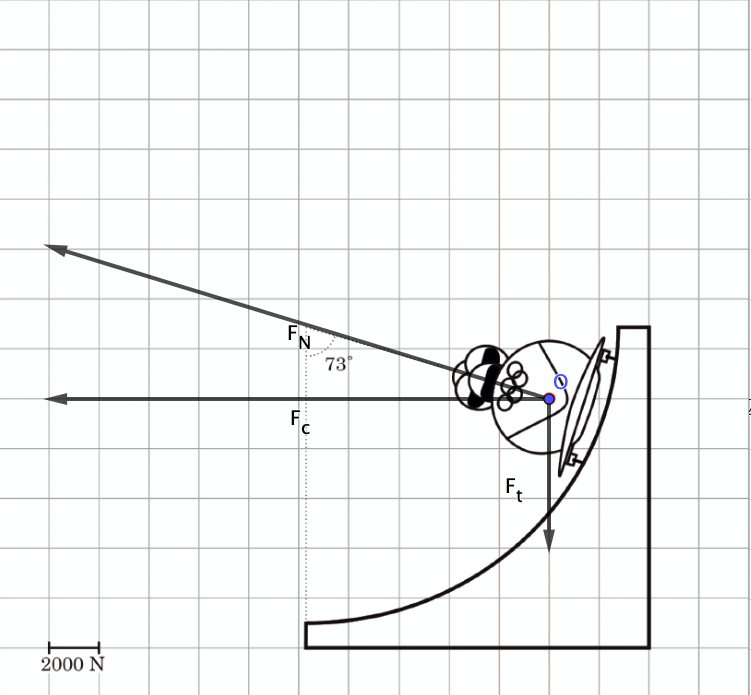
\includegraphics[scale=0.5]{bobslæde.png}
\end{center}
\caption{Repræsentanter for kræfterne indtegnet i GeoGebra}
\label{fig:bob}
\end{figure}
Vi kan finde et udtryk for $v$ ud fra udtrykket for centripetalkraften. 
\begin{equation*}
\begin{split}
  |\overrightarrow{\textbf{F}_c}|=m \cdot \frac{v^2}{r} &\iff v=\sqrt{\frac{|\overrightarrow{\textbf{F}_c}| \cdot r}{m}} \\
  &\iff v=\sqrt{\frac{|\overrightarrow{\textbf{F}_N}| \cdot \sin\left(73 \degree \right) \cdot r}{m}} 
\end{split}
\end{equation*}
Vi kan nu regne farten ud.
\begin{equation*}
\begin{split}
  v&=\sqrt{\frac{|\overrightarrow{\textbf{F}_N}| \cdot \sin\left(73 \degree \right) \cdot r}{m}} \\
  &=\sqrt{\frac{21160,05 \;\unit{N} \cdot \sin\left(73 \degree \right) \cdot 20 \;\unit{m} }{630 \;\unit{kg} }} \\
  &\approx 25 \;\unit{m/s} 
\end{split}
\end{equation*}
Bobslædens fart i cirkelbevægelsen er altså $25 \;\unit{m/s} $.
\section*{Accelerationssensor}
\sol \\
\textbf{a.}
Omløbstiden udregnes.
\begin{equation*}
\begin{split}
  T&=\frac{1}{f}\\
  &=\frac{1}{78 \;\unit{min^{-1}} }\\
  &=\frac{1}{78} \cdot 60\;\unit{s} \\
  &\approx 0,77 \;\unit{s} 
\end{split}
\end{equation*}
Omløbstiden i cirkelbevægelsen er altså $0,77 \;\unit{s} $.\\[1ex]
\textbf{b.}
Data fra tabellen sat ind i et regneark med lineær regression ses i \cref{fig:plade}.
\begin{figure}[H]
\begin{center}
  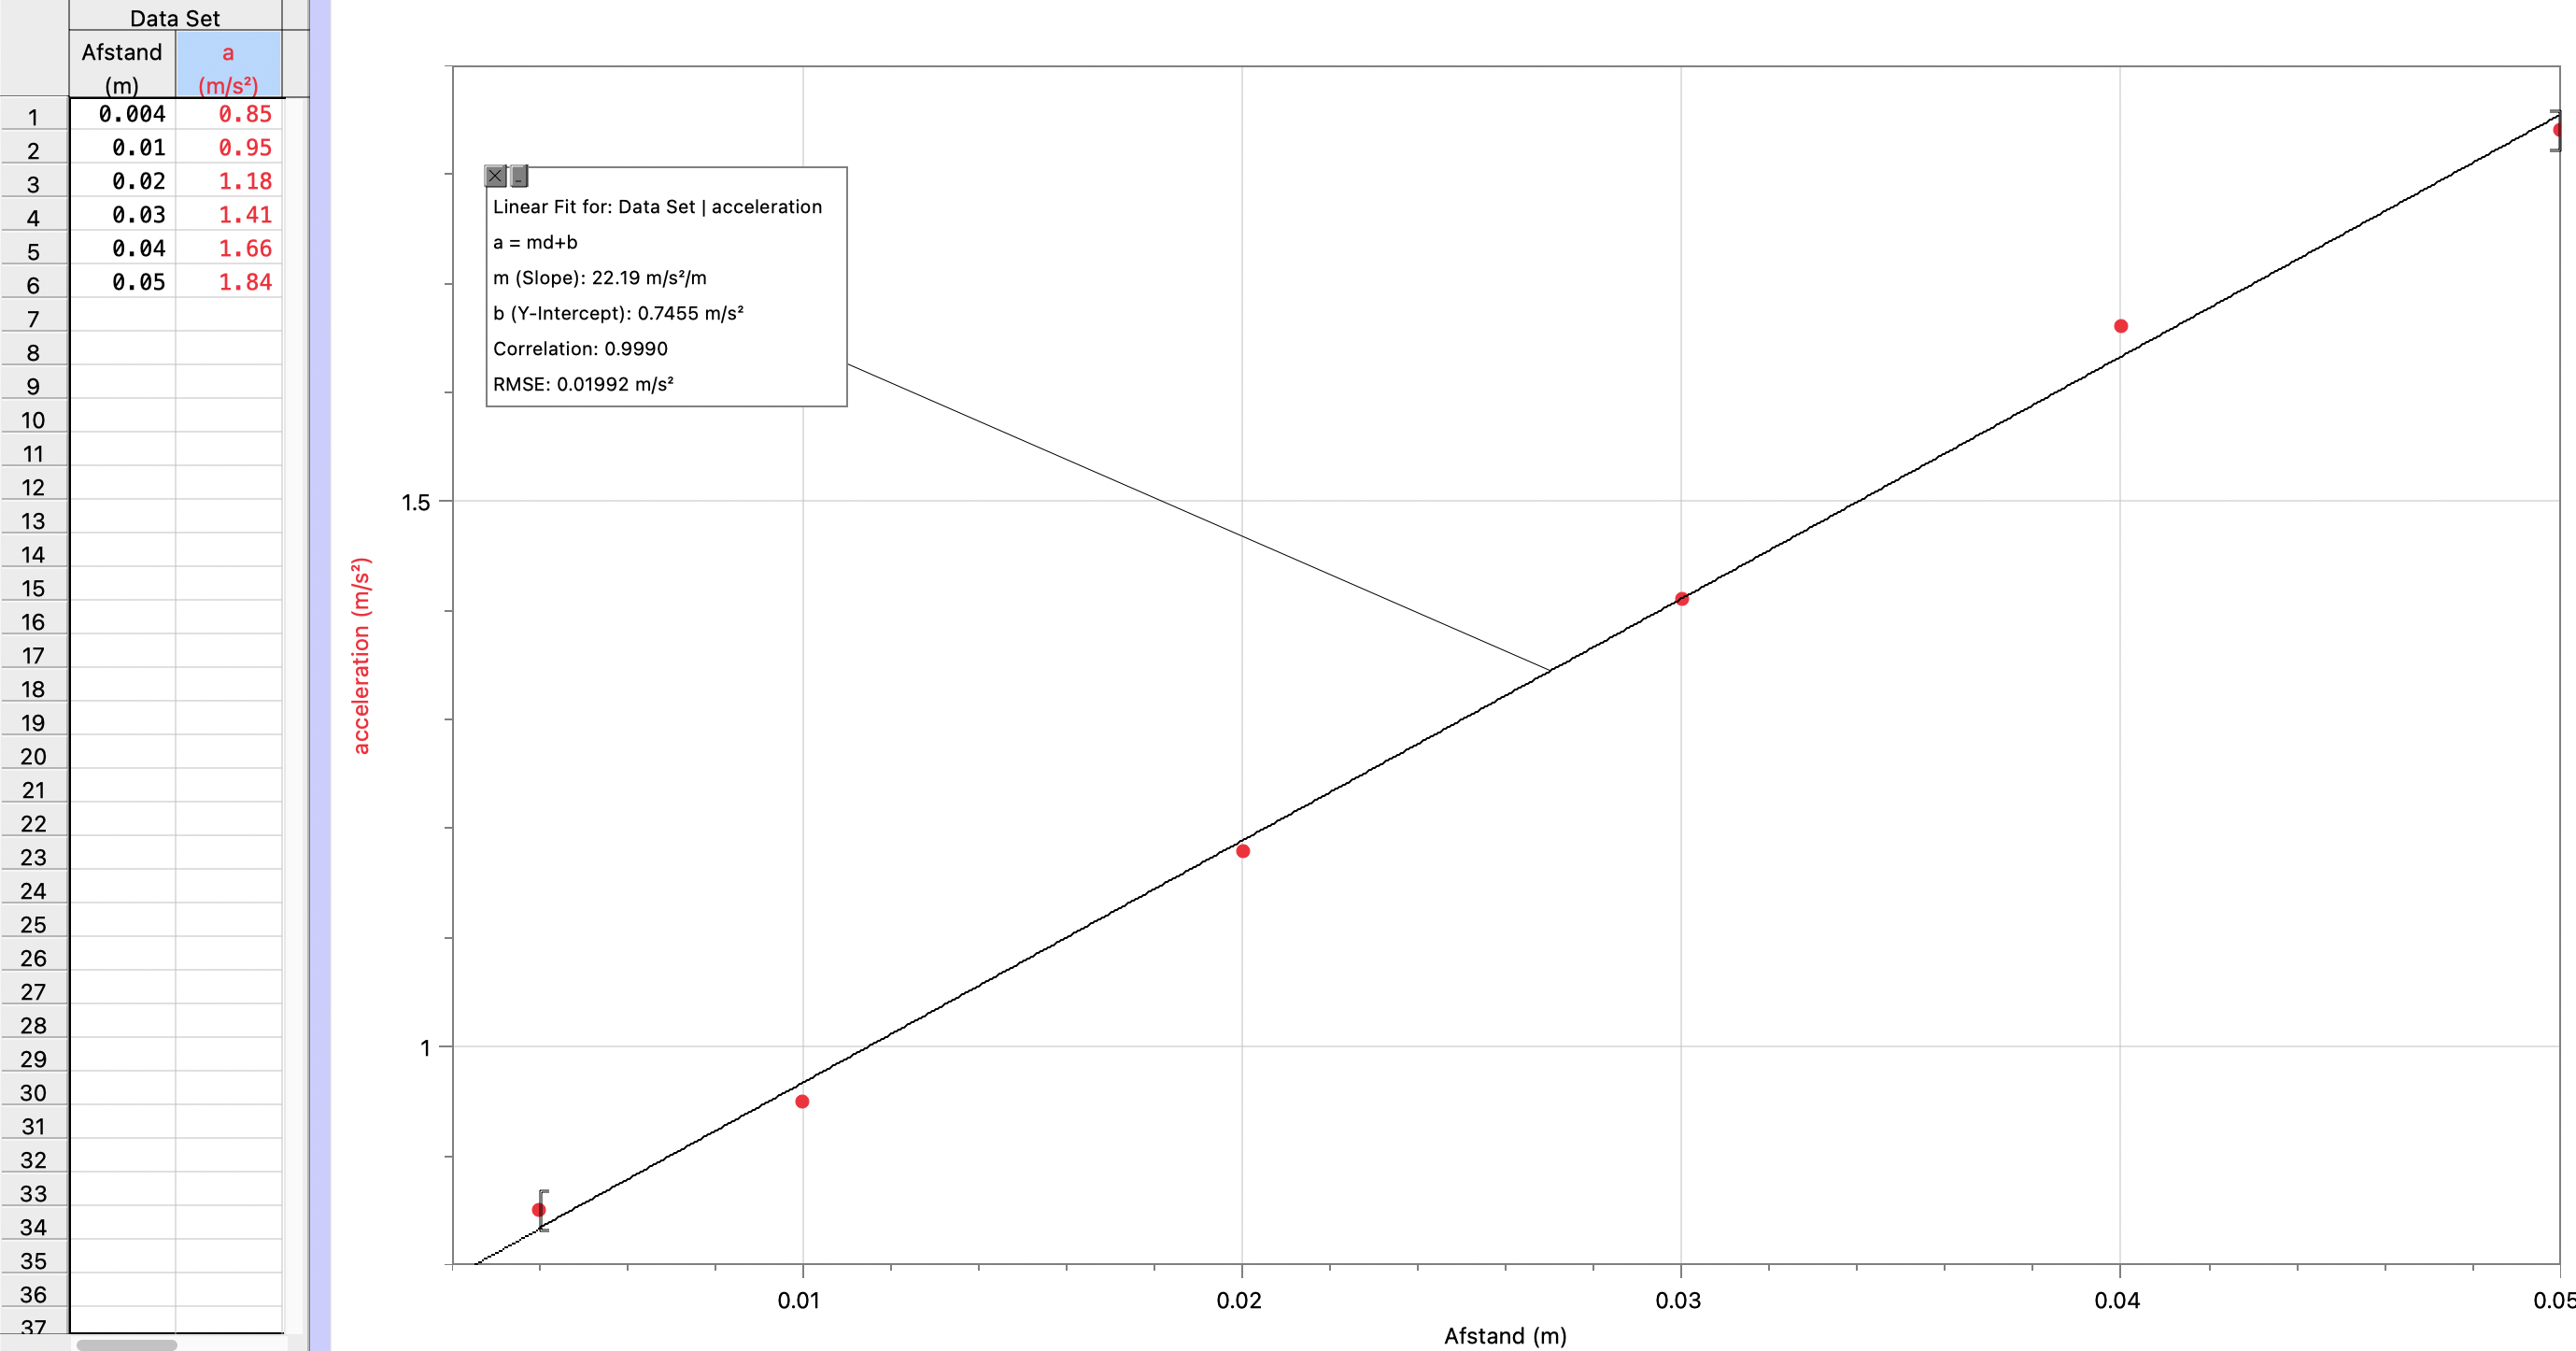
\includegraphics[scale=0.3]{plade.png}
\end{center}
\caption{Lineær regression lavet i Logger Pro}
\label{fig:plade}
\end{figure}
Lad $x$ betegne afstanden fra accelerationssensoren til mobiltelefonens kant nærmest centrum af pladespilleren.
Så har vi
\begin{equation}
\label{1}
\begin{split}
  a_c&=\omega^2 \cdot r\\
  &=\omega^2 \cdot (d+x)\\
  &=\omega^2 \cdot d + \omega^2 \cdot x
\end{split}
\end{equation}
Fra regressionen har vi
\begin{equation}
  \label{2}
\begin{split}
a_c=22,19 \;\unit{s^{-2}} \cdot d + 0,7455 \;\unit{m/s^2} 
\end{split}
\end{equation}
Altså må der gælde, at
\[
\omega^2=22,19 \;\unit{s ^{-2}} 
\] 
Imidlertid gælder der også, at
\begin{equation*}
\begin{split}
  \omega=2 \cdot \pi \cdot f &\iff f=\frac{\omega }{2 \pi }\\
  &\iff f=\frac{\sqrt{\omega^2} }{2 \pi }
\end{split}
\end{equation*}
da $\omega>0 $.
Vi regner nu frekevensen ud.
\begin{equation*}
\begin{split}
  f&=\frac{\sqrt{\omega^2} }{2 \pi }\\
  &=\frac{\sqrt{22,19 \;\unit{s ^{-2}} }  }{2 \pi }\\
  &\approx 0,7 \;\unit{Hz} 
\end{split}
\end{equation*}
Fra ligning \ref{1} og \ref{2} har vi, at
\begin{equation*}
\begin{split}
  \omega^2 \cdot x=0,7455 \;\unit{m/s^2} \iff x=\frac{0,7455 \;\unit{m/s^2} }{\omega^2}
\end{split}
\end{equation*}
Vi beregner nu $x$.
\begin{equation*}
\begin{split}
  x&=\frac{0,7455 \;\unit{m/s^2} }{22,19 \;\unit{s ^{-2}} }\\
  &\approx 0,03 \;\unit{m} \\
  &=3 \;\unit{cm} 
\end{split}
\end{equation*}
Vi har altså fået frekevensen til at være $0,7 \;\unit{Hz} $ og afstanden fra accelerationssensoren til mobiltelefonens kant nærmest centrum af pladespilleren til at være $3 \;\unit{cm} $. 
\section*{Stangtennis}
Vi antager, at pigens højde er $1,6 \;\unit{m} $.
Snoren ser ud til at være præcis halvt så lang som pigen og dens længde må da være $\frac{1,60 \;\unit{m} }{2}=0,80 \;\unit{m} $.
Med vinkelmåler måles det, at snoren danner $80 \degree$ med vandret, og vi antager også, at der er tale om en jævn cirkelbevægelse.
Cirklens radius $r$ må da være
\begin{equation*}
\begin{split}
  r=0,80 \;\unit{m} \cdot \sin\left(80 \degree  \right)
\end{split}
\end{equation*}
Altså må den resulterende kraft $\overrightarrow{\textbf{F}_c} $ have retning vandret mod centrum. 
Siden $\overrightarrow{\textbf{F}_c} = \overrightarrow{\textbf{F}_N}+\overrightarrow{\textbf{F}_t} $, så må $\overrightarrow{\textbf{F}_N}$'s komposant i $y$-retningen være lige stor og modsatrettet $\overrightarrow{\textbf{F}_t}$. 
Ved at betragte en retvinklet trekant er det nemt at se, at
\begin{equation*}
\begin{split}
  |\overrightarrow{\textbf{F}_c}|&=|\overrightarrow{\textbf{F}_t}| \cdot \tan\left(80 \degree \right) 
\end{split}
\end{equation*}
Hvis vi kombinerer dette med et andet udtryk for centripetalkraften får vi , at
\begin{equation*}
\begin{split}
  |\overrightarrow{\textbf{F}_c}|=m \cdot \frac{v^2}{r} &\iff v=\sqrt{\frac{r \cdot|\overrightarrow{\textbf{F}_c}|}{m}} \\
  &\iff v=\sqrt{\frac{r \cdot|\overrightarrow{\textbf{F}_t}| \cdot \tan\left(80 \degree \right)  }{m}} \\
  &\iff v=\sqrt{r \cdot g \cdot \tan\left(80 \degree \right)  } \\
\end{split}
\end{equation*}
Vi regner nu farten ud.
\begin{equation*}
\begin{split}
  v&=\sqrt{r \cdot g \cdot \tan\left(80 \degree \right)  } \\
  &=\sqrt{0,80 \;\unit{m} \cdot \sin\left(80 \degree \right) \cdot 9,82 \;\unit{m/s^2} \cdot \tan\left(80 \degree \right)  } \\
  &\approx 6,6 \;\unit{m/s} 
\end{split}
\end{equation*}
Tennisboldens fart i situationen på billedet er altså $6,6 \;\unit{m/s} $.
\end{document}
